%! TeX root = ./main.tex
% vim: set spelllang=fr:
\selectlanguage{french}
\chapter{Approches algébriques pour la réconciliation segmentale}\label{chap:adp-rec}

\newcommand{\algsignrec}{\algsign_{\mathrm{rec}}}
\newcommand{\gramrec}{\gram_{\mathrm{rec}}}
\newcommand{\gRec}{\mathrm{Rec}}
\newcommand{\gRecPath}{\mathrm{Rec}^{\downarrow}}
\newcommand{\gRecIn}{\mathrm{Rec}^{\ast}}
\newcommand{\gRecOut}{\mathrm{Rec}^{\curvearrowright}}
\newcommand{\xmin}{x_{\mathrm{min}}}
\newcommand{\xin}{x_{\mathrm{in}}}
\newcommand{\xout}{x_{\mathrm{out}}}
\newcommand{\xlca}{x_{\mathrm{lca}}}
\newcommand{\algsignset}{\algsign_{\mathrm{set}}}
\newcommand{\evSplit}{\mathrm{split}}
\newcommand{\gramset}{\gram_{\mathrm{set}}}
\newcommand{\gCont}{\mathrm{C}}
\newcommand{\gContSub}{\mathrm{\Delta}}
\newcommand{\gSplit}{\mathrm{Split}}
\newcommand{\gBranch}{\mathrm{Branch}}
\newcommand{\gramseq}{\gram_{\mathrm{seq}}}
\newcommand{\gRecSplit}{\mathrm{RecSplit}}
\newcommand{\gRecPathBranch}{\mathrm{RecBranch}^{\downarrow}}
\newcommand{\gRecInBranch}{\mathrm{RecBranch}^{\ast}}
\newcommand{\gRecOutBranch}{\mathrm{RecBranch}^{\curvearrowright}}
\newcommand{\gRecBranchEnd}{\mathrm{RecBranch}'}

\tikzset{
    unary/.code n args={3}{
        \pgfkeysalso{#1}
        \def\cmp{#2}\ifx\cmp\empty\else
            \pgfkeysalso{
                label={[%
                    font={\scriptsize\vphantom{gb}},
                    label distance=3pt,
                    inner xsep=0pt, inner ysep=0pt,
                    outer xsep=0pt, outer ysep=0pt,
                ]#3:#2},
            }
        \fi
    },
    gain/.style n args={3}{
        unary={
            draw={#1}, fill=black,
            semicircle, inner sep=1pt,
        }{#2}{#3},
    },
    loss/.style n args={3}{
        unary={
            draw={#1}, fill=black,
            semicircle, inner sep=1pt,
            shape border rotate={180},
        }{#2}{#3},
    },
}

Le problème de réconciliation segmentale peut être vu comme une combinaison de deux problèmes indépendants: d’une part celui de la réconciliation bilatérale de l’arbre des synténies avec l’arbre des hôtes, et d’autre part celui de l’inférence des groupes de contenus ancestraux des synténies.
Dans ce chapitre, nous montrons que l’approche algébrique présentée au \cref{chap:adp} permet de rendre cette intuition précise et concrète.
Nous faisons indépendamment un traitement algébrique de chacun des deux problèmes dans les \cref{sec:adp-rec:bilateral,sec:adp-rec:set} puis nous montrons comment combiner leurs solutions pour résoudre la réconciliation segmentale dans la \cref{sec:adp-rec:both}.

\section{Réconciliation bilatérale}\label{sec:adp-rec:bilateral}

Afin de résoudre le \cref{prob:reconciliation:parsimony} de \(\recmodelDTLx\)-parcimonie pour la réconciliation bilatérale par l’approche algébrique, nous développons dans cette section une grammaire décrivant l’espace des solutions ainsi qu’une collection d’algèbres permettant d’évaluer ces solutions.
Pour rappel, l’entrée de ce problème est composée d’un arbre d’unités \(T\), d’un arbre d’hôtes \(S\), ainsi que d’une application \(\llmap : \tleavs(T) \onto \tleavs(S)\) associant chaque unité actuelle de \(T\) à son hôte de \(S\).
L’objectif est d’identifier les réconciliations qui possèdent les interprétations les plus parcimonieuses, c’est-à-dire les arbres réconciliés qui expliquent l’entrée en utilisant le moins d’événements possible.

Nous fixons pour signature du problème, au sens de la \cref{def:adp:alg}, l’ensemble d’opérateurs \(\algsignrec = \{\algnull, \algplus, \evLeaf, \evSkip, \evSpe, \evDup, \evTr\}\) définis comme suit:
\begin{itemize}
    \item \(\evLeaf_{t,v}\) représente une unité actuelle \(t \in \tleavs(T)\) dont l’hôte est \(v \in \tleavs(S)\);
    \item \(\evSkip_n(h)\) représente un saut vers un descendant à distance \(n\) de l’hôte actuel, interprétable comme une succession de \(n\) événements \(\evtS\) et \(\evtL\), ou comme un seul événement \(\evtTX\);
    \item \(\evSpe_{t,v}(h_L, h_R)\), \(\evDup_{t,v}(h_L, h_R)\) et \(\evTr_{t,v}(h_L, h_R)\) représentent respectivement des événements de type \(\evtS\), \(\evtD\) et \(\evtT\) concernant l’unité \(t \in \tnodes(T)\) associée à l’hôte \(v \in \tnodes(S)\).
\end{itemize}

Cette signature permet de représenter n’importe quel ensemble d’arbres réconciliés parcimonieux sous le modèle~\(\recmodelDTLx\) et ainsi de représenter l’espace des solutions du problème considéré.

\subsection{Algèbres d’évaluation}

Pour toute fonction de coûts \(\cost : \recmodelDTLx \onto \realpos \cup \{\infty\}\), nous pouvons définir l’algèbre d’optimisation~\(\alminplus_\cost\) suivante respectant la signature~\(\algsignrec\):\\
\sidecols{.5\textwidth}{.5\textwidth}{
\begin{align*}
    \algnull &= \infty \\
    \algplus &= \min \\
    \evLeaf_{t,v} &= 0 \\
    \evSpe_{t,v}(h_L, h_R) &= h_L + h_R
\end{align*}
}{
\begin{align*}
    \evDup_{t,v}(h_L, h_R) &= h_L + h_R + \cost(\evtD) \\
    \evTr_{t,v}(h_L, h_R) &= h_L + h_R + \cost(\evtT) \\
    \evSkip_{n}(h) &= h + \min\{n\cost(\evtL), \cost(\evtTX)\}. \\
\end{align*}
}

Cette algèbre est additive et peut donc être convertie en algèbre de Boltzmann (voir \cref{sec:adp:space-enum-sample}) afin de réaliser un échantillonnage des solutions optimales et quasioptimales.

Comme avec toute signature, une algèbre de traçage \(\altrace(\algsignrec)\) peut être construite afin de construire les circuits algébriques représentant l’espace de solutions associé à une certaine entrée (voir \cref{sec:adp:solution-spaces:trace}).
Cela permet, par exemple, de construire automatiquement l’ensemble des solutions de coût minimum, en utilisant l’algèbre combinée \(\alminplus_\cost \times \altrace(\algsignrec) \mid \allex{1}\).

En l’absence d’une fonction de coûts fixée, il peut être souhaitable de réaliser une optimisation multiobjectifs, en construisant des ensembles de vecteurs Pareto-optimaux de la forme \(\tup{n_\evtD, n_\evtT, n_\evtL, n_\evtTX}\) dénombrant le nombre d’événements de chaque type.
Cette tâche est compliquée par le fait que l’opérateur \(\evSkip_n(h)\) peut être interprété soit comme une série d’événements~\(\evtL\), soit comme un seul événement~\(\evtTX\), selon le coût relatif de ces deux événements.
Chaque appel à \(\evSkip_n(h)\) doit ainsi engendrer deux vecteurs représentant ces deux interprétations possibles, ce qui nous empêche d’employer la construction générique de la \cref{sec:adp:alg-combin:pareto}.
Nous construisons donc manuellement l’algèbre comme suit: \\
\sidecols{.35\textwidth}{.65\textwidth}{
\begin{align*}
    \algnull &= \emptyset \\
    h \algplus h' &= \parfront(h \cup h') \\
    \evLeaf_{t,v} &= \{\tup{0, 0, 0, 0}\} \\
    \evSpe_{t,v}(h_L, h_R) &= \parfront(h_L + h_R) \\[-3.2ex]
\end{align*}
}{
\begin{align*}
    \evDup_{t,v}(h_L, h_R) &= \parfront(h_L + h_R + \{\tup{1, 0, 0, 0}\}) \\
    \evTr_{t,v}(h_L, h_R) &= \parfront(h_L + h_R + \{\tup{0, 1, 0, 0}\}) \\
    \evSkip_n(h) &= \begin{cases}
        h & \text{si } n = 0 \\
        \parfront(h + \{\tup{0, 0, n, 0}, \tup{0, 0, 0, 1}\}) & \text{sinon,}
    \end{cases}
\end{align*}
}\\
où \enquote{\(+\)} correspond à une somme de Minkowski, construisant l’ensemble des sommes des paires de vecteurs obtenues en prenant le produit cartésien des deux opérandes.

\subsection{Grammaire de structure}

L’espace des réconciliations a été formellement étudié par plusieurs auteurs, notamment \textcite{Doyon2009SpaceGeneSpeciesTrees} pour le modèle \(\recmodelDL\).
Plus récemment, \textcite{Chauve2020CountingSamplingGene} ont proposé une grammaire décrivant l’espace des arbres réconciliés sous le modèle \(\recmodelDTL\), sans contrainte sur l’arbre des unités.
Dans cette section, nous proposons une grammaire canonique pour l’espace des réconciliations sous le modèle \(\recmodelDTLx\).

La grammaire \(\gramrec\), présentée selon les conventions de la \cref{sec:adp:yield-gram}, utilise quatre prédicats représentant chacun un ensemble de réconciliations possibles du sous-arbre \(T\) donné dans leur première dimension.
Ces prédicats sont définis ainsi:
\begin{compactitemize}
    \item \(\gRec[T, S]\): réconciliations telles que \(\troot(T)\) est appariée à \(\troot(S)\);
    \item \(\gRecOut[T, S]\): telles que \(\troot(T)\) est appariée à n’importe quel hôte \(s \nottcomp \troot(S)\);
    \item \(\gRecIn[T, S]\): telles que \(\troot(T)\) est appariée à n’importe quel hôte \(s \tdesc \troot(S)\);
    \item \(\gRecPath[T, S, 0]\): telles que \(\troot(T)\) est appariée à n’importe quel hôte \(s \tdesc \troot(S)\) et précédée d’un événement \(\evSkip_N\) avec \(N = \tdist(s, \troot(S))\).
\end{compactitemize}
L'espace des solutions pour deux phylogénies \(T\) et \(S\) est engendré par \(\gRecIn[T, S]\).\\
Les clauses de la grammaire sont:
{\allowdisplaybreaks
\begin{subequations}
\begin{align}
    \gRec[t(), v()] &\rightarrow \evLeaf_{t,v}
    \qquad\text{\itshape\small (seulement lorsque \(\llmap(t) = v\))} \label{eq:adp-rec:bilateral-grammar-leaf}\\[2ex]
    \gRec[t((T') \mid (T'')), v((S_L)(S_R))] &\rightarrow
        \evSpe_{t,v}(\gRecPath[(T'), (S_L), 0], \gRecPath[(T''), (S_R), 0]) \label{eq:adp-rec:bilateral-grammar-spe} \\
    \gRec[t((T_L)(T_R)), v(S)] &\rightarrow
        \evDup_{t,v}(\gRecPath[(T_L), v(S), 0], \gRecPath[(T_R), v(S), 0]) \label{eq:adp-rec:bilateral-grammar-dup} \\
    \gRec[t((T') \mid (T'')), v(S)] &\rightarrow
        \evTr_{t,v}(\gRecOut[(T'), v(S)], \gRecPath[(T''), v(S), 0]) \label{eq:adp-rec:bilateral-grammar-tr} \\[2ex]
    \gRecPath[T, v((S') \mid S''), N] &\rightarrow \gRecPath[T, S', N+1] \label{eq:adp-rec:bilateral-grammar-path-down}\\
    \gRecPath[T, S, N] &\rightarrow \evSkip_N(\gRec[T, S]) \label{eq:adp-rec:bilateral-grammar-path-end}\\
    \gRecIn[T, v((S') \mid S'')] &\rightarrow \gRecIn[T, S'] \label{eq:adp-rec:bilateral-grammar-in-down}\\
    \gRecIn[T, S] &\rightarrow \gRec[T, S] \label{eq:adp-rec:bilateral-grammar-in-end}\\[2ex]
    \gRecOut[T, S \text{ frère de } S'] &\rightarrow
        \gRecIn[T, S'] \label{eq:adp-rec:bilateral-grammar-out-side}\\
    \gRecOut[T, P \text{ parent de } S] &\rightarrow
        \gRecOut[T, P] \label{eq:adp-rec:bilateral-grammar-out-up}
\end{align}
\end{subequations}}%
Suivant les conventions de la \cref{sec:adp:yield-gram}, la notation \((T')\mid(T'')\) indique que \(T'\) et \(T''\) sont les deux sous-arbres enfants de la racine, pris dans n’importe quel ordre, alors que la notation \((T_L)(T_R)\) indique que l’ordre de l’entrée est conservé.

Les clauses \labelcref{eq:adp-rec:bilateral-grammar-spe,eq:adp-rec:bilateral-grammar-dup,eq:adp-rec:bilateral-grammar-tr} agissent au niveau des embranchements de l’arbre \(T\) pour y insérer des événements de cospéciation, de duplication ou de transfert.

Les clauses \labelcref{eq:adp-rec:bilateral-grammar-path-down,eq:adp-rec:bilateral-grammar-path-end,eq:adp-rec:bilateral-grammar-in-down,eq:adp-rec:bilateral-grammar-in-end} traversent les hôtes descendants d’un certain sommet,
soit en tenant compte du nombre de sommets traversé pour insérer un appel à \(\evSkip_N\)~(\(\gRecPath\)),
soit en poursuivant directement avec une réconciliation au niveau du descendant, comme au début d’une réconciliation ou à la suite d’un événement de transfert~(\(\gRecIn\)).

Finalement, les clauses \labelcref{eq:adp-rec:bilateral-grammar-out-side,eq:adp-rec:bilateral-grammar-out-up} permettent de traverser les hôtes séparés d’un certain sommet.
Elles s’appuient sur le principe récursif selon lequel un sommet séparé de \(v\) est soit un descendant d’un frère de~\(v\), soit un sommet séparé du parent de \(v\).
Ce principe a été employé par \textcite{Bansal2012EfficientAlgorithmsReconciliation} pour réduire la complexité de l’algorithme de \(\recmodelDTL\)-parcimonie d’un facteur \(|\tnodes(S)|\).

Nous conjecturons que cette grammaire est non ambigüe et qu’elle est canonique pour le problème de \(\recmodelDTLx\)-parcimonie dans le sens où chaque réconciliation parcimonieuse possible pour une entrée donnée est énumérée exactement une fois.

Grâce à l’\cref{alg:seq-yield-parser}, cette grammaire correspond automatiquement à un algorithme de programmation dynamique.
Sa complexité en temps est \(\bigo(nmd)\)\footnote{Cette complexité ne prend en compte que le temps de construction du circuit algébrique associé à une certaine entrée. En fonction de l’algèbre utilisée pour évaluer ce circuit, la complexité totale pourrait être plus élevée. Dans le cas où seul le coût minimum d’une solution, ou seule la construction d’une solution arbitraire atteignant ce coût, sont recherchés, la complexité est exactement telle qu’indiqué.}, où \(n\) et \(m\) sont les tailles de \(T\) et \(S\) et \(d\) est la profondeur de \(S\), en vertu du \cref{thm:adp:gram-hedge-complex}.
Cette complexité est proche de la meilleure complexité connue pour le problème de réconciliation bilatérale \parencite{Weiner2021ImprovedDuplicationTransfer}, à un facteur \(d\) près.
Ce facteur peut toutefois être éliminé en supprimant le paramètre \(N\) du prédicat \(\gRecPath\), en insérant à la place un appel à \(\evSkip_1\) à chaque application de la clause \labelcref{eq:adp-rec:bilateral-grammar-path-down}, et en ajoutant une clause séparée pour inférer les événements \(\evtTX\).
Cependant, cette transformation rend la grammaire non canonique, puisqu’il existe alors toujours deux solutions partielles connectant deux sommets de~\(T\), l’une empruntant une série d’appels à \(\evSkip\), l’autre la nouvelle clause pour les événements \(\evtTX\).

Il est possible d’étendre cette grammaire pour résoudre le problème de binarisation d’un arbre \(T\) contenant des polytomies de sorte à minimiser le coût de réconciliation \(\recmodelDTLx\) associé.
La complexité de l’algorithme résultant, en vertu du \cref{thm:adp:gram-forest-complex}, est \(\bigo(n^22^{\deg I})\), c’est-à-dire qu’il s’agit d’un algorithme \emph{fixed parameter tractable} (FPT) dans le degré maximum de l’arbre des unités.
Cette complexité est comparable à celle de l’algorithme développé par \textcite{Kordi2016ExactAlgorithmsDuplicationTransferLoss}.

\subsection{Résultats}

L’application de la grammaire \(\gramrec\) sur l’entrée à gauche de la \cref{fig:adp-rec:rec-input} engendre un certain espace de solutions, sous la forme d’un circuit algébrique sur lequel différentes algèbres peuvent être appliquées.
Ce circuit algébrique correspond au \emph{graphe de réconciliation} étudié notamment par \textcite{Scornavacca2013RepresentingSetReconciliations,Wang2022EfficientlySparseListing}.
L’\cref{alg:adp:circ-sample} pour l’échantillonnage de solutions appliqué à ce graphe correspond exactement à celui développé par \textcite{Bansal2013ReconciliationRevisitedHandling} spécifiquement pour le problème de réconciliation.

En utilisant l’algèbre~\(\alminplus_\cost\) avec un coût de \(\cost(\evtD) = 2\), \(\cost(\evtT) = 3\), \(\cost(\evtL) = 1\) et \(\cost(\evtTX) = \infty\), nous obtenons un coût minimal de~10.
En combinant cette algèbre avec l’algèbre de traçage \(\altrace(\algsignrec)\) grâce au combinateur lexicographique décrit à la \cref{sec:adp:alg-combin:lex}, il est possible de construire la solution atteignant ce coût présentée à droite de la \cref{fig:adp-rec:rec-input}.
En construisant une algèbre de Pareto, nous pouvons obtenir le diagramme de la \cref{fig:adp-rec:rec-pareto}, qui montre qu’il existe plusieurs classes de solutions parcimonieuses obtenues en faisant varier les différents paramètres de coûts.

\begin{figure}[p]
    \capstart
    \centering
    %! TeX root = ../../main.tex
% vim: set spelllang=fr:
\begin{tikzpicture}
    \begin{scope}[xscale=-1]
        \graph[
            phylogenetic tree layout,
            nodes={font=\small\bfseries},
            evolutionary unit length=1cm,
        ]{
            s1 / [coordinate, label={[yshift=2pt]left:\(s_1\)}] -- {
                s2 / [coordinate, label={left:\(s_2\)}] -- {
                    1,
                    2,
                },
                s3 / [coordinate, label={right:\(s_3\)}] -- {
                    3,
                    4,
                },
            },
        };
        \node at (0, -2.8) {\(S\)};
    \end{scope}

    \begin{scope}[shift={(-4.25,0)},xscale=-1]
        \graph[
            phylogenetic tree layout,
            nodes={font=\small\itshape},
            evolutionary unit length=.5cm,
        ]{
            t1 / [coordinate, label={[yshift=2pt]left:\(t_1\)}] -- {
                t2 / [coordinate, label={left:\(t_2\)}] -- {
                    t3 / [coordinate, label={left:\(t_3\)}] -- {
                        t4 / [coordinate, label={left:\(t_4\)}] -- {
                            l1s4 / 1,
                            l1s3 / 3,
                        },
                        l2s4 / 2 [> length=2],
                    },
                    l2s6 / 4 [> length=3],
                },
                t5 / [coordinate, label={right:\(t_5\)}] -- {
                    l1s2 / 1 [> length=3],
                    t6 / [coordinate, label={right:\(t_6\)}] -- {
                        l1s1 / 4 [> length=2],
                        l1s0 / 4 [> length=2],
                    },
                },
            },
        };
        \node at (.2, -2.8) {\(T\)};
    \end{scope}

    \draw[separator rule] (2, -2.9) -- ++(0, 3);

    \begin{scope}[shift={(3,-2.6)}]
        \tikzset{
    x={(1pt,0)},
    y={(0,-1pt)},
    limit width/.style 2 args={
        execute at begin node={\begin{varwidth}{#1}#2},
        execute at end node={\end{varwidth}},
    },
    host background/.style={
        fill=host background color,
        draw=host background color,
        line width={.01pt},
    },
    unsampled host background/.style={
        preaction={fill=host background color},
        draw=host background color,
        pattern={Lines[angle=45, distance=3pt, line width=1.5pt]},
        pattern color=white,
    },
    host label/.style={
        font=\bfseries,
        midway,
        anchor=north,
        limit width={12em}{\centering},
    },
    branch/.style={
        draw={#1},
        line width={0.5pt},
    },
    loss branch/.style={
        branch,
        draw={black!40},
    },
    transfer branch/.style={
        branch={#1},
        densely dashed,
        -{Latex[length=0pt 8]},
    },
    invalid transfer branch/.style={
        transfer branch={red!80!black},
        out distance=20,
        in distance=20,
    },
    event/.style={
        draw={#1}, fill={host background color!50!white},
        font={\color{#1}},
        outer sep=0pt, inner xsep=0pt, inner ysep=2pt,
        limit width={6em}{\narrowragged},
        line width={0.5pt},
    },
    event/.default={black},
    extant/.code 2 args={
        \pgfkeysalso{
            circle, fill={#1},
            outer sep=0pt, inner sep=0pt,
            minimum size={3},
        }
        \def\cmp{#2}\ifx\cmp\empty\else
            \pgfkeysalso{
                label={[%
                    font={\color{#1}\vphantom{gb}},
                    fill=host background color!35!white,
                    rounded corners=2,
                    label distance=2pt,
                    inner xsep=2pt, inner ysep=1pt,
                    outer xsep=0pt, outer ysep=0pt,
                    limit width={6em}{\centering},
                ]below:#2},
            }
        \fi
    },
    extant/.default={black}{},
    unsampled/.style={
        circle, fill={#1},
        outer sep=0pt, inner sep=0pt,
        minimum size={3},
    },
    unsampled/.default={black!40},
    speciation/.style 2 args={
        event={#1}, rectangle, rounded corners,
        inner xsep=4pt,
        minimum width={8},
        minimum height={8},
        execute at begin node={#2},
    },
    duplication/.style 2 args={
        event={#1}, rectangle,
        inner xsep=4pt,
        minimum width={8},
        minimum height={8},
        execute at begin node={#2},
    },
    transfer/.code 2 args={
        \pgfkeysalso{
            event={#1},
        }
        \def\cmp{#2}\ifx\cmp\empty
            \pgfkeysalso{
                diamond,
                inner sep=1.5pt,
            }
        \else
            \pgfkeysalso{
                chamfered rectangle,
                chamfered rectangle sep={8 / 2.4},
                inner xsep=2pt,
                inner ysep=-1pt,
                minimum width={8},
                minimum height={8},
                execute at begin node={#2},
            }
        \fi
    },
    gain/.code 2 args={
        \pgfkeysalso{
            draw={#1}, fill=black,
            semicircle, inner sep=1pt,
            shape border rotate={0},
        }
        \def\cmp{#2}\ifx\cmp\empty\else
            \pgfkeysalso{
                label={[%
                    font={\scriptsize\vphantom{gb}},
                    label distance=2pt,
                    inner xsep=0pt, inner ysep=0pt,
                    outer xsep=0pt, outer ysep=0pt,
                    limit width={6em}{\narrowragged},
                ]right:#2},
            }
        \fi
    },
    loss/.code 2 args={
        \pgfkeysalso{
            draw={#1}, fill=black,
            semicircle, inner sep=1pt,
            shape border rotate={180+0},
        }
        \def\cmp{#2}\ifx\cmp\empty
            \pgfkeysalso{draw={black!40}, fill={black!40}}
        \else
            \pgfkeysalso{
                label={[%
                    font={\scriptsize\vphantom{gb}},
                    label distance=2pt,
                    inner xsep=0pt, inner ysep=0pt,
                    outer xsep=0pt, outer ysep=0pt,
                    limit width={6em}{\narrowragged},
                ]right:#2},
            }
        \fi
    },
}
% hosts
\path[host background] (0.0,-18.0) [rounded corners={2pt}] to (0.0,1.0) to node[host label] {1} (18.0,1.0) [sharp corners] to (18.0,-18.0) -- cycle;
\path[host background] (30.75,-13.0) [rounded corners={2pt}] to (30.75,1.0) to node[host label] {2} (47.6222,1.0) [sharp corners] to (47.6222,-13.0) -- cycle;
\path[host background] (0.0,-9.0) [rounded corners={2pt}] to (0.0,-44.0) to (13.5,-44.0) [sharp corners] to (13.5,-48.0) to (35.25,-48.0) [rounded corners={2pt}] to (35.25,-44.0) to (47.6222,-44.0) [sharp corners] to (47.6222,-6.5) to (30.75,-6.5) [rounded corners={2pt}] to (30.75,-18.0) to (18.0,-18.0) [sharp corners] to (18.0,-9.0) -- cycle;
\path[host background] (51.6222,-13.5) [rounded corners={2pt}] to (51.6222,1.0) to node[host label] {3} (76.3665,1.0) [sharp corners] to (76.3665,-13.5) -- cycle;
\path[host background] (88.1804,-17.5) [rounded corners={2pt}] to (88.1804,1.0) to node[host label] {4} (109.1804,1.0) [sharp corners] to (109.1804,-17.5) -- cycle;
\path[host background] (51.6222,-6.75) [rounded corners={2pt}] to (51.6222,-44.0) to (70.9304,-44.0) [sharp corners] to (70.9304,-48.0) to (92.6804,-48.0) [rounded corners={2pt}] to (92.6804,-44.0) to (109.1804,-44.0) [sharp corners] to (109.1804,-8.75) to (88.1804,-8.75) [rounded corners={2pt}] to (88.1804,-18.0) to (76.3665,-18.0) [sharp corners] to (76.3665,-6.75) -- cycle;
\path[host background] (13.5,-33.0) [rounded corners={2pt}] to (13.5,-74.0) to (42.2152,-74.0) [sharp corners] to (42.2152,-82.5) to (63.9652,-82.5) [rounded corners={2pt}] to (63.9652,-74.0) to (92.6804,-74.0) [sharp corners] to (92.6804,-33.0) to (70.9304,-33.0) [rounded corners={2pt}] to (70.9304,-48.0) to (35.25,-48.0) [sharp corners] to (35.25,-33.0) -- cycle;
% unsampled hosts
% branches
\path[branch] (7.5,-13.5) to (7.5,-4.5);
\path[transfer branch] (7.5,-13.5) to (56.1222,-13.5);
\path[branch] (20.75,-25.25) [rounded corners={1.5pt}] to (7.5,-25.25) [sharp corners] to (7.5,-13.5);
\path[branch] (20.75,-25.25) [rounded corners={1.5pt}] to (35.25,-25.25) [sharp corners] to (35.25,-4.5);
\path[branch] (28.0,-36.75) [rounded corners={1.5pt}] to (13.5,-36.75) [sharp corners] to (13.5,-4.5);
\path[loss branch] (28.0,-36.75) [rounded corners={1.5pt}] to (42.1861,-36.75) [sharp corners] to (42.1861,-4.4361);
\path[branch] (56.1222,-13.5) to (56.1222,-4.5);
\path[branch] (101.6804,-13.25) [rounded corners={1.5pt}] to (98.6804,-13.25) [sharp corners] to (98.6804,-4.5);
\path[branch] (101.6804,-13.25) [rounded corners={1.5pt}] to (104.6804,-13.25) [sharp corners] to (104.6804,-4.5);
\path[branch] (78.1804,-25.25) [rounded corners={1.5pt}] to (92.6804,-25.25) [sharp corners] to (92.6804,-4.5);
\path[loss branch] (78.1804,-25.25) [rounded corners={1.5pt}] to (63.0582,-25.25) [sharp corners] to (63.0582,-4.4361);
\path[branch] (85.4304,-36.75) [rounded corners={1.5pt}] to (101.6804,-36.75) [sharp corners] to (101.6804,-13.25);
\path[loss branch] (85.4304,-36.75) [rounded corners={1.5pt}] to (70.9304,-36.75) [sharp corners] to (70.9304,-4.4361);
\path[branch] (49.4652,-55.25) [rounded corners={1.5pt}] to (20.75,-55.25) [sharp corners] to (20.75,-25.25);
\path[branch] (49.4652,-55.25) [rounded corners={1.5pt}] to (78.1804,-55.25) [sharp corners] to (78.1804,-25.25);
\path[branch] (56.7152,-66.75) [rounded corners={1.5pt}] to (28.0,-66.75) [sharp corners] to (28.0,-36.75);
\path[branch] (56.7152,-66.75) [rounded corners={1.5pt}] to (85.4304,-66.75) [sharp corners] to (85.4304,-36.75);
\path[branch] (53.0902,-78.25) [rounded corners={1.5pt}] to (49.4652,-78.25) [sharp corners] to (49.4652,-55.25);
\path[branch] (53.0902,-78.25) [rounded corners={1.5pt}] to (56.7152,-78.25) [sharp corners] to (56.7152,-66.75);
% gene transfers
% events
\node[extant={black}{}] at (7.5,-4.5) {};
\node[transfer={black}{}] at (7.5,-13.5) {};
\node[extant={black}{}] at (13.5,-4.5) {};
\node[extant={black}{}] at (35.25,-4.5) {};
\node[loss={black}{}] at (42.1861,-4.4361) {};
\node[speciation={black}{}] at (20.75,-25.25) {};
\node[speciation={black}{}] at (28.0,-36.75) {};
\node[extant={black}{}] at (56.1222,-4.5) {};
\node[loss={black}{}] at (63.0582,-4.4361) {};
\node[loss={black}{}] at (70.9304,-4.4361) {};
\node[extant={black}{}] at (92.6804,-4.5) {};
\node[extant={black}{}] at (98.6804,-4.5) {};
\node[extant={black}{}] at (104.6804,-4.5) {};
\node[duplication={black}{}] at (101.6804,-13.25) {};
\node[speciation={black}{}] at (78.1804,-25.25) {};
\node[speciation={black}{}] at (85.4304,-36.75) {};
\node[speciation={black}{}] at (49.4652,-55.25) {};
\node[speciation={black}{}] at (56.7152,-66.75) {};
\node[duplication={black}{}] at (53.0902,-78.25) {};

    \end{scope}
\end{tikzpicture}

    \caption[Instance et solution à un problème de \(\recmodelDTLx\)-parcimonie]{
        \emph{(Gauche.)} Exemple d’instance \((T, S)\) du problème de \(\recmodelDTLx\)-parcimonie.
        \emph{(Droite.)} Unique solution optimale pour un coût de \(\cost(\evtD) = 2\), \(\cost(\evtT) = 3\), \(\cost(\evtL) = 1\) et \(\cost(\evtTX) = \infty\).
        Voir les légendes des \cref{fig:reconciliation:strict-rec,fig:reconciliation:rec-trees} pour les explications de lecture.
        \label{fig:adp-rec:rec-input}
    }
\end{figure}

\begin{table}[p]
    \capstart
    \centering
    \scalebox{.95}{\begin{tabular}{cccccccccc}
\toprule
\multirow{2}{*}[-2pt]{\(\tnodes(T)\)} &
\multirow{2}{*}[-2pt]{Ev.} &
\multicolumn{7}{c}{\(\tnodes(S)\)} &
\multirow{2}{*}[-2pt]{Total} \\
\cmidrule(lr){3-9}
&& \(1\) & \(2\) & \(3\) & \(4\) & \(s_1\) & \(s_2\) & \(s_3\) & \\
\midrule
\multirow{3}{*}{\(t_1\)} & \(\evtS\) & --- & --- & --- & --- & 0.26881 & 0.01333 & 0.00496 & 0.28709 \\
& \(\evtD\) & 0.00076 & --- & --- & 0.01724 & 0.58096 & 0.01334 & 0.02343 & 0.63573 \\
& \(\evtT\) & 0.01700 & 0.00154 & 0.00063 & 0.01649 & --- & 0.02058 & 0.02094 & 0.07718 \\
\midrule
\multirow{3}{*}{\(t_2\)} & \(\evtS\) & --- & --- & --- & --- & 0.49449 & --- & 0.13429 & 0.62878 \\
& \(\evtD\) & --- & --- & --- & --- & 0.01676 & --- & 0.00738 & 0.02414 \\
& \(\evtT\) & 0.00393 & 0.02215 & 0.00860 & 0.09818 & --- & 0.15349 & 0.06074 & 0.34708 \\
\midrule
\multirow{3}{*}{\(t_3\)} & \(\evtS\) & --- & --- & --- & --- & 0.00593 & 0.71103 & --- & 0.71697 \\
& \(\evtD\) & --- & --- & --- & --- & 0.00133 & 0.02605 & --- & 0.02737 \\
& \(\evtT\) & 0.02092 & 0.06239 & 0.14932 & --- & --- & 0.01781 & 0.00521 & 0.25566 \\
\midrule
\multirow{3}{*}{\(t_4\)} & \(\evtS\) & --- & --- & --- & --- & 0.00109 & --- & --- & 0.00109 \\
& \(\evtD\) & --- & --- & --- & --- & 0.00002 & --- & --- & 0.00002 \\
& \(\evtT\) & 0.77138 & --- & 0.19432 & --- & --- & 0.01308 & 0.02011 & 0.99889 \\
\midrule
\multirow{3}{*}{\(t_5\)} & \(\evtS\) & --- & --- & --- & --- & 0.48863 & --- & --- & 0.48863 \\
& \(\evtD\) & --- & --- & --- & --- & 0.00984 & --- & --- & 0.00984 \\
& \(\evtT\) & 0.16584 & --- & --- & 0.10924 & --- & 0.12263 & 0.10383 & 0.50153 \\
\midrule
\multirow{3}{*}{\(t_6\)} & \(\evtS\) & --- & --- & --- & --- & --- & --- & --- & --- \\
& \(\evtD\) & --- & --- & --- & 0.80298 & 0.00089 & --- & 0.19613 & 1.00000 \\
& \(\evtT\) & --- & --- & --- & --- & --- & --- & --- & --- \\
\bottomrule
\end{tabular}
}
    \caption[Probabilités d’occurrence des événements dans un scénario moyen]{
        Probabilités d’occurrence des événements dans un scénario moyen de la distribution de Boltzmann avec température \(T=1\) pour l’entrée et les coûts de la \cref{fig:adp-rec:rec-input}.
        Le tableau indique la probabilité que chaque sommet de \(T\) soit assigné à un certain type d’événement parmi \(\evtS\), \(\evtD\) ou \(\evtT\) et soit associé à un certain hôte de l’arbre~\(S\).
        \label{fig:adp-rec:rec-supports}
    }
\end{table}

\begin{figure}[htbp]
    \capstart
    \centering
    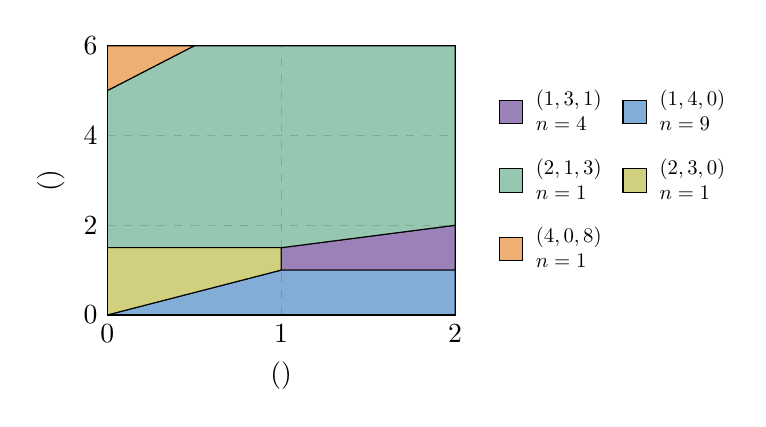
\begin{tikzpicture}
    \definecolor{c0}{HTML}{6F4C9B}
    \definecolor{c1}{HTML}{4D8AC6}
    \definecolor{c2}{HTML}{69B190}
    \definecolor{c3}{HTML}{BEBC48}
    \definecolor{c4}{HTML}{E78C35}
    \pgfplotsset{layers/mosaic/.define layer set={axis background,pre main,main,lines,marks,axis grid,axis ticks,axis lines,axis tick labels,axis descriptions,axis foreground}{/pgfplots/layers/standard}}
    \pgfplotsset{set layers=mosaic}
    \begin{axis}[
        width=6cm,
        height=5cm,
        clip mode=individual,
        legend style={
            anchor=west,
            at={(1.1, 0.5)},
            cells={anchor=west, align=left},
            nodes={scale=.75, transform shape},
            draw=none,
            column sep=3pt,
            /tikz/every even column/.append style={column sep=6pt},
            row sep=6pt,
        },
        legend columns=2,
        grid=both,
        grid style={black, opacity=.15, dashed},
        tick style={transparent},
        xtick distance=1,
        ytick distance=2,
        enlargelimits=false,
        xlabel={\(\cost(\evtD)\)},
        ylabel={\(\cost(\evtT)\)},
        area legend/.style={
            legend image code/.code={
                \draw [#1] (0cm,-0.15cm) rectangle (0.3cm,0.15cm);
            }, 
        },
    ]
    \addplot[area legend, black, fill=c0!70!white, mark=none] coordinates { (1.0, 1.0) (1.0, 1.5) (2.0, 2.0) (2.0, 1.0) (1.0, 1.0) };
    \addlegendentry{\((1, 3, 1)\)\\\(n=4\)}
    \addplot[area legend, black, fill=c1!70!white, mark=none] coordinates { (0.0, 0.0) (1.0, 1.0) (2.0, 1.0) (2.0, 0.0) (0.0, 0.0) };
    \addlegendentry{\((1, 4, 0)\)\\\(n=9\)}
    \addplot[area legend, black, fill=c2!70!white, mark=none] coordinates { (0.0, 1.5) (0.0, 5.0) (0.5, 6.0) (2.0, 6.0) (2.0, 2.0) (1.0, 1.5) (0.0, 1.5) };
    \addlegendentry{\((2, 1, 3)\)\\\(n=1\)}
    \addplot[area legend, black, fill=c3!70!white, mark=none] coordinates { (0.0, 0.0) (0.0, 1.5) (1.0, 1.5) (1.0, 1.0) (0.0, 0.0) };
    \addlegendentry{\((2, 3, 0)\)\\\(n=1\)}
    \addplot[area legend, black, fill=c4!70!white, mark=none] coordinates { (0.0, 5.0) (0.0, 6.0) (0.5, 6.0) (0.0, 5.0) };
    \addlegendentry{\((4, 0, 8)\)\\\(n=1\)}
    \end{axis}
\end{tikzpicture}

    \caption[Mosaïque des régions de coûts pour une instance de \(\recmodelDTLx\)-parcimonie]{
        Mosaïque des régions d’optimalité des coûts selon trois dimensions: nombre d’événements de duplication, de transfert et de perte.
        Les scénarios parcimonieux contenant des événements \(\evtTX\) sont écartés de ce diagramme.
        Celui-ci montre la tranche de l’espace des coûts pour \(\cost(\evtL) = 1\).
        La région \(\tup{2, 1, 3}\) contient la solution de la \cref{fig:adp-rec:rec-input}.
        \label{fig:adp-rec:rec-pareto}
    }
\end{figure}

Finalement, il est possible d’échantillonner des solutions quasioptimales en construisant une algèbre de Boltzmann comme décrit à la \cref{ex:adp:space-enum-sample:boltz}.
De cet ensemble peuvent être calculées efficacement les probabilités que chaque embranchement de \(T\) soit assigné à un événement donné ou à un hôte donné dans une solution moyenne (voir \cref{fig:adp-rec:rec-supports}) au travers du calcul des contributions externes introduit à la \cref{sec:adp:space-enum-sample:outside}, généralisant ainsi l’approche développée par~\textcite{Nguyen2013SupportMeasuresEstimate}.

\section{Parcimonie de groupes}\label{sec:adp-rec:set}

Le problème de la parcimonie de groupes, sous-jacent à la réconciliation segmentale, concerne l’inférence du contenu ancestral de synténies dans un arbre dont le contenu aux feuilles est connu.
Cette inférence s’appuie sur un modèle de gains et de pertes groupés, de sorte que chaque arête de l’arbre peut être étiquetée par un événement de gain qui fait apparaître simultanément une ou plusieurs nouvelles unités ou par une perte qui en fait disparaître.
Nous prendrons l’hypothèse de~Dollo, selon laquelle chaque unité est gagnée exactement une fois.

L’objectif du problème est de trouver un étiquetage de contenus ancestraux le plus parcimonieux en termes de gains et de pertes, en fonction du nombre d’événements et de leurs tailles respectives.
Plus précisément, chaque embranchement doit être étiqueté par un groupe de sorte à minimiser le coût formé par la somme, sur chaque branche \((v, v\child)\), de \(\cost_\evtG(|\syntenyOfExt(v\child) - \syntenyOfExt(v)|)\) et \(\cost_\evtL(|\syntenyOfExt(v) - \syntenyOfExt(v\child)|)\).
Un exemple d’instance pour le problème est présenté à la \cref{fig:adp-rec:set-example}.

\begin{problem}{Parcimonie de groupes}
    \probinput{Phylogénie \(T\);
               ensemble d’unités \(\geneFamilySet\);
               étiquetage \(\syntenyOf : \tleavs(T) \onto 2^{\geneFamilySet}\);\newline
               coûts \(\cost_\evtG, \cost_\evtL : \nat \onto \realpos\).}
    \proboutput{Affectation \(\syntenyOfExt : \tnodes(T) \onto 2^{\geneFamilySet}\) étendant \(\syntenyOf\) de coût minimum.}
\end{problem}

\begin{figure}[h]
    \capstart
    \centering
    %! TeX root = ../../main.tex
% vim: set spelllang=fr:
\begin{tikzpicture}[xscale=-1]
    \begin{scope}
        \graph[
            phylogenetic tree layout,
            evolutionary unit length=0.7cm,
            nodes={font=\small\strut, inner sep=0pt},
            length=1,
        ]{
            tf / [coordinate] -- {
                tc / [coordinate] -- {
                    tb / [coordinate] -- {
                        ta / [coordinate] -- {
                            t1 / b,
                            t2 / bc,
                        },
                        t3 / bce [>length=2],
                    },
                    t4 / ac [>length=3],
                },
                te / [coordinate] -- {
                    t5 / abd [>length=3],
                    td / [coordinate] -- {
                        t6 / bdf [>length=2],
                        t7 / bdfg [>length=2],
                    },
                },
            }
        };
    \end{scope}
    \draw[separator rule] (-3.2, -3) -- ++(0, 3);
    \begin{scope}[shift={(-7.5, 0)}]
        \graph[
            phylogenetic tree layout,
            evolutionary unit length=0.7cm,
            nodes={font=\small\strut, inner ysep=0pt},
            length=1,
        ]{
            tf / abcdef -- {
                tc / abcdef -- {
                    tb / bce [>edge node={node [loss={black}{adf}{left}] {}}] -- {
                        ta / bce -- {
                            t1 / b [>edge node={node [loss={black}{ce}{left}] {}}],
                            t2 / bc [>edge node={node [loss={black}{e}{right}] {}}],
                        },
                        t3 / bce [>length=2],
                    },
                    t4 / ac [>length=3, >edge node={node [loss={black}{bdef}{right}] {}}],
                },
                te / abcdef -- {
                    t5 / abd [>length=3, >edge node={node [loss={black}{cef}{right}] {}}],
                    td / bdf [>edge node={node [loss={black}{ace}{right}] {}}] -- {
                        t6 / bdf [>length=2],
                        t7 / bdfg [>length=2, >edge node={node [gain={black}{g}{right}] {}}],
                    },
                },
            }
        };
        \draw (tf) edge node[gain={black}{abcdef}{right}] {} ($(tf)+(0,.66)$);
    \end{scope}
\end{tikzpicture}

    \caption[Instance et solution à un problème de parcimonie de groupes]{
        \emph{(Gauche.)} Exemple d’entrée pour le problème de parcimonie de groupes.
        Chaque feuille est étiquetée par un ensemble d’unités chacune représentée par une lettre différente.
        L’ordre dans lequel celles-ci sont inscrites est sans importance.
        Cet exemple est tiré de \textcite{Gascon2026GeneRepertoireEvolution}.
        \emph{(Droite.)} Une solution possible pour l’entrée donnée.
        Les événements de gain sont représentés par des demi-cercles ouverts vers le bas et ceux de perte par des demi-cercles ouverts vers le haut, à côté desquels le groupe d’unités gagnées ou perdues est indiqué.
        \label{fig:adp-rec:set-example}
    }
\end{figure}

Une première version du problème a été étudiée par \textcite{Delabre2020EvolutionSegmentalDuplications} en ignorant la taille des pertes et en supposant que toutes les unités soient gagnées dès la racine de l’arbre.
Au cours du printemps~2025, Corélie~\textsc{Godefroid} a étudié la version de ce problème étendue pour également placer les événements de gains de manière optimale.
Ces idées ont été développées par Mathieu~\textsc{Gascon}, menant à un article présenté à la conférence RECOMB-CG~2026 \parencite{Gascon2026GeneRepertoireEvolution}.
La solution présentée dans la suite de cette section est basée sur ce travail.

\subsection{Réduction du problème}

Observons que ce problème peut être vu comme portant sur la taille des groupes ancestraux et non sur leur contenu.
En effet, puisque les fonctions de coûts considérées dépendent uniquement du nombre d’événements de gain et de perte et du nombre d’unités gagnées et perdues, deux solutions qui infèrent les mêmes tailles de groupes ancestraux sont indistinguables du point de vue de leur coût et seront considérées comme équivalentes dans la suite.
Le problème se rapproche ainsi de celui résolu par le programme Count de \textcite{Csuros2010CountEvolutionaryAnalysis} qui infère des profils de nombre de copies ancestrales d’une famille de gènes sur la base d’un modèle probabiliste.

Certaines contraintes existent toutefois sur les tailles des groupes ancestraux.
À chaque embranchement \(v \in \tnodes(T)\), l’ensemble des unités~\(\geneFamilySet\) peut être partitionné en trois sous-ensembles \(\geneFamilySet = \xmin(v) \cup \xin(v) \cup \xout(v)\), où:
\begin{compactitemize}
    \item \(\xmin(v)\) est l’ensemble des unités dont le \emph{lca} est un ancêtre de \(v\) et qui apparaissent dans au moins une feuille du sous-arbre de \(v\);
    \item \(\xout(v)\) est l’ensemble des unités qui n’apparaissent dans aucune feuille du sous-arbre de \(v\);
    \item \(\xin(v)\) est l’ensemble des unités dont le \emph{lca} est un descendant strict de \(v\).
\end{compactitemize}
En raison de l’hypothèse de Dollo, les unités de \(\xmin(v)\) apparaissent dans l’ensemble \(\syntenyOfExt(v)\) dans toute solution.
À l’inverse, \(\xout(v)\) et \(\xin(v)\) contiennent des unités qui peuvent y apparaître de manière optionnelle: dans le cas de \(\xout(v)\), celles-ci peuvent être librement perdues dans la branche menant à \(v\) et, dans le cas de \(\xin(v)\), elles peuvent y être librement gagnées.

Pour représenter l’espace des solutions du problème, nous fixons donc pour signature l’ensemble d’opérateurs \(\algsignset = \{\algnull,\allowbreak \algplus,\allowbreak \evLeaf,\allowbreak \evGain,\allowbreak \evLoss,\allowbreak \evSplit\}\) définis comme suit:
\begin{itemize}
    \item \(\evLeaf\) représente une feuille de l’arbre;
    \item \(\evGain_N(h)\) et \(\evLoss_N(h)\) représentent respectivement un gain ou une perte de \(N\) unités;
    \item \(\evSplit_{G_L,G_R,L}(h_L, h_R)\) représente un embranchement de l’arbre au niveau duquel \(G_L+G_R\) unités restent à gagner, dont \(G_L\) dans le sous-arbre à gauche et \(G_R\) dans le sous-arbre à droite, et \(L\) unités restent à perdre.
\end{itemize}

\subsection{Algèbres d’évaluation}

Cette signature permet, pour deux fonctions de coûts \(\cost_\evtG\) et \(\cost_\evtL\) données, de définir l’algèbre d’optimisation additive \(\alminplus_{\cost_\evtG,\cost_\evtL}\) suivante\\
\threecols{.33\textwidth}{.33\textwidth}{.33\textwidth}{
\begin{align*}
    \algnull &= \infty \\
    \evGain_N(h) &= h + \cost_\evtG(N)
\end{align*}
}{
\begin{align*}
    \algplus &= \min \\
    \evLoss_N(h) &= h + \cost_\evtL(N)
\end{align*}
}
{
\begin{align*}
    \evLeaf &= 0 \\
    \evSplit_{G,G',L}(h_L, h_R) &= h_L + h_R.
\end{align*}
}

Comme précédemment, cette algèbre peut être adaptée en algèbre de Boltzmann ou de Pareto.

Notons que les fonctions \(\cost_\evtG\) et \(\cost_\evtL\) peuvent être arbitraires.
Un coût constant, c’est-à-dire de la forme \(\cost_e(n) = b_e\) si \(n \ge 1\) et \(0\) sinon, pour une constante \(b_e \in \realpos \cup \{\infty\}\), permet de minimiser le nombre d’événements sans prendre en compte la taille des gains et des pertes.
Le problème devient alors équivalent au problème sous-jacent à la réconciliation segmentale de \textcite{Delabre2020EvolutionSegmentalDuplications} et des \cref{chap:superdtl,chap:synesth}.
Les solutions obtenues avec ces coûts ont tendance à regrouper beaucoup d’événements et à engendrer une quantité excessive de pertes.

Un coût linéaire, c’est-à-dire de la forme \(\cost_e(n) = a_en\) pour une constante \(a_e \in \realpos \cup \{\infty\}\), permet de rechercher les solutions minimisant la taille totale des événements.
Il rend cependant le problème équivalent à la parcimonie de Dollo individuelle, puisque les unités peuvent alors être considérées comme évoluant indépendamment.

Plus généralement, un coût affine de la forme \(\cost_e(n) = a_en + b_e\) si \(n \ge 1\) et \(0\) sinon, pour deux constantes \(a_e, b_e \in \realpos \cup \{\infty\}\), prend simultanément en compte la dépendance entre les unités étudiées tout en accordant une préférence aux solutions plus parcimonieuses minimisant globalement la taille des événements.
Dans la suite, les constantes \(b_e\) sont appelées les coûts d’ouverture et les constantes \(a_e\) les coûts d’extension des gains ou des pertes.

\subsection{Grammaire de structure}

L’espace des solutions peut être décrit par une grammaire \(\gramset\) de dimension trois.
La première dimension \(T\) représente le sous-arbre traité.
La seconde dimension \(G\) représente le nombre d’unités restant à gagner dans le sous-arbre traité.
La troisième dimension \(L\) représente le nombre d’unités de l’ensemble \(\xout\) présentes, c’est-à-dire qui ont déjà été gagnées mais qui n’apparaissent dans aucune feuille du sous-arbre traité.
La grammaire utilise trois prédicats définis ainsi:
\begin{compactitemize}
    \item \(\gSplit[T, G, L]\) représente les solutions dont la racine est \(T\) et en dessous de laquelle il reste à gagner \(G\) unités et à en perdre \(L\);
    \item \(\gBranch[T, G, L]\) et \(\gBranch'[T, G, L]\) représentent les solutions qui ajoutent des événements unaires de perte et de gain au-dessus de \(T\).
\end{compactitemize}
À chaque niveau de la solution, il faut s’assurer que \(G\) ne dépasse pas le nombre d’unités qui peuvent être potentiellement gagnées dans le sous-arbre traité.
Plus précisément, pour chaque embranchement \(v\), notons \(\xlca(v)\) l’ensemble qui rassemble toutes les unités dont le \(\lca\) est un descendant de \(v\), c’est-à-dire les unités qui peuvent être gagnées en \(v\) ou en dessous.
Chaque appel à l’un des trois prédicats n’amène ainsi à une solution valide que si \(G \le |\xlca(v)|\).

L’ensemble des solutions est constitué des termes dérivés de \(\gBranch[T, |\geneFamilySet|, 0]\), où \(T\) est l’arbre d’entrée et \(\geneFamilySet\) l’ensemble de toutes les unités.
Les clauses de la grammaire sont:
{\allowdisplaybreaks
\begin{subequations}
\begin{align}
    \gSplit[(), 0, 0] &\rightarrow \evLeaf \label{eq:adp-rec:set-split-leaf} \\[2ex]
    \begin{aligned}
        &\gSplit[t(t\lchild(T_L)\,t\rchild(T_R)), G_L + G_R, L] \\
        \rightarrow\ & \evSplit_{G_L, G_R, L}(
            \begin{aligned}[t]
                &\gBranch[t\lchild(T_L), G_L, L + |\xlca(t\rchild)| - G_R + |\xmin(t) - \xmin(t\lchild)|], \\
                &\gBranch[t\rchild(T_R), G_R, L + |\xlca(t\lchild)| - G_L + |\xmin(t) - \xmin(t\rchild)|])
            \end{aligned} \\
        &\text{\itshape\small (seulement lorsque \(|\xlca(t\lchild)| \ge G_L\) and \(|\xlca(t\rchild)| \ge G_R\))}
    \end{aligned} \span \label{eq:adp-rec:set-split-inner}\\[2ex]
    \gBranch[T, G, L_H + L_D] &\rightarrow \evLoss_{L_H}(\gBranch'[T, G, L_D]) \label{eq:adp-rec:set-split-loss}\\
    \gBranch'[T, G_H + G_D, L] &\rightarrow \evGain_{G_H}(\gSplit[T, G_D, L]). \label{eq:adp-rec:set-split-gain}
\end{align}
\end{subequations}}%
La clause \labelcref{eq:adp-rec:set-split-inner} s’applique à chaque embranchement de \(T\).
Chacune des \(G\) unités qui restent à gagner à un certain embranchement peuvent être gagnés soit dans le sous-arbre gauche, soit dans le sous-arbre droit, d’où la décomposition en \(G = G_L + G_R\).
Chacune des \(L\) unités qui sont issues de l’ensemble \(\xout(t)\) sont par définition éléments des ensembles \(\xout(t\lchild)\) et \(\xout(t\rchild)\), auxquels il faut ajouter les unités qui seront gagnées de l’autre côté (resp. \(|\xmin(t) - \xmin(t\lchild)|\) et \(|\xmin(t) - \xmin(t\rchild)|\)) et celles qui ont déjà été gagnées mais ne sont plus nécessaires dans le sous-arbre actuel (resp. \(|\xlca(t\rchild)| - G_R\) et \(|\xlca(t\lchild)| - G_L\)).

Les clauses \labelcref{eq:adp-rec:set-split-loss,eq:adp-rec:set-split-gain} introduisent respectivement une perte et un gain d’un nombre d’unités au plus égal à la valeur courante de \(L\) ou de \(G\).

Nous conjecturons que cette grammaire est non ambigüe et qu’elle est canonique pour le problème de parcimonie de groupes, c’est-à-dire que chaque scénario est énuméré exactement une fois, en considérant uniquement la taille des groupes et non leur contenu exact.

Grâce à l’\cref{alg:seq-yield-parser}, cette grammaire correspond automatiquement à un algorithme de programmation dynamique.
En vertu du \cref{thm:adp:gram-hedge-complex}, sa complexité en temps est \(\bigo(nf^3)\), où \(n\) est la taille de \(T\) et \(f\) le nombre d’unités dans \(\geneFamilySet\).
Le fait de séparer les deux clauses \labelcref{eq:adp-rec:set-split-loss,eq:adp-rec:set-split-gain} est nécessaire pour conserver une complexité en \(f^3\) au lieu de \(f^4\).

Les solutions de l’espace de solutions ainsi engendré ne décrivent pas directement le contenu des groupes ancestraux, mais seulement leurs tailles respectives.
Cependant, il est aisé de déterminer un exemple de contenu pour toute solution en utilisant les ensembles \(\xmin(v)\), \(\xin(v)\) et \(\xout(v)\).

\subsection{Résultats}

L’application de la grammaire \(\gramset\) sur l’entrée à gauche de la \cref{fig:adp-rec:set-example} engendre un certain espace de solutions sur lequel différentes algèbres peuvent être appliquées.
En utilisant l’algèbre~\(\alminplus_{\cost_\evtG,\cost_\evtL}\) avec un coût constant, nous obtenons un nombre d’événements minimal de~8.
En combinant cette algèbre avec l’algèbre de traçage \(\altrace(\algsignset)\) grâce au combinateur lexicographique, il est possible de construire la solution atteignant ce coût présentée à droite de la \cref{fig:adp-rec:set-example}.

L’utilisation d’un coût affine fixant le coût d’ouverture des gains et des pertes à \(b_\evtL = b_\evtG = 3\) et leur coût d’extension à \(a_\evtL = a_\evtG = 1\) permet d’identifier la solution présentée à gauche de la \cref{fig:adp-rec:set-solutions}.
Avec l’algèbre de Pareto, nous pouvons construire le diagramme de la \cref{fig:adp-rec:set-pareto} qui montre qu’il existe plusieurs classes de solutions parcimonieuses obtenues en faisant varier les différents paramètres de coûts.

Finalement, il est possible d’échantillonner des solutions quasioptimales en construisant une algèbre de Boltzmann comme décrit à la \cref{ex:adp:space-enum-sample:boltz}.
Cet ensemble peut être caractérisé en calculant l’espérance de la taille des groupes ancestraux au travers du calcul des contributions externes introduit à la \cref{sec:adp:space-enum-sample:outside}, comme présenté à droite de la \cref{fig:adp-rec:set-solutions}.

\begin{figure}[p]
    \capstart
    \centering
    \begin{tikzpicture}[xscale=-1]
    \begin{scope}
        \graph[
            phylogenetic tree layout,
            evolutionary unit length=0.95cm,
            nodes={font=\small\strut, inner ysep=0pt},%, draw, rounded corners},
            length=1,
        ]{
            tf / abd -- {
                tc / abcd [>edge node={node [gain={black}{c}{left}] {}}] -- {
                    tb / bc [>edge node={node [loss={black}{ad}{left}] {}}] -- {
                        ta / bc -- {
                            t1 / b [>edge node={node [loss={black}{c}{left}] {}}],
                            t2 / bc,
                        },
                        t3 / bce [>length=2, >edge node={node [gain={black}{e}{right}] {}}],
                    },
                    t4 / ac [>length=3, >edge node={node [loss={black}{bd}{right}] {}}],
                },
                te / abd -- {
                    t5 / abd [>length=3],
                    td / bdf [
                        >edge node={node [pos=.25, loss={black}{a}{right}] {}},
                        >edge node={node [pos=.7, gain={black}{f}{right}] {}},
                    ] -- {
                        t6 / bdf [>length=2],
                        t7 / bdfg [>length=2, >edge node={node [gain={black}{g}{right}] {}}],
                    },
                },
            }
        };
        \draw (tf) edge node[gain={black}{abd}{right}] {} ($(tf)+(0,.66)$);
    \end{scope}

    \draw[separator rule] (-3.6, -4.2) -- ++(0, 4.8);
    \begin{scope}[shift={(-8,0)}]
        % temp=1, gain=loss=3, ext=1
        % 1
        % loss=1.044
        % gain=0.000
        % size=1.000

        % 2
        % loss=0.044
        % gain=0.000
        % size=2.000

        % A
        % loss=0.160
        % gain=0.000
        % size=2.044

        % 3
        % loss=0.050
        % gain=0.846
        % size=3.000

        % B
        % loss=1.570
        % gain=0.025
        % size=2.204

        % 4
        % loss=1.748
        % gain=0.000
        % size=2.000

        % C
        % loss=0.117
        % gain=0.706
        % size=3.748

        % 5
        % loss=0.467
        % gain=0.000
        % size=3.000

        % 6
        % loss=0.369
        % gain=0.000
        % size=3.000

        % 7
        % loss=0.087
        % gain=0.718
        % size=4.000

        % D
        % loss=1.123
        % gain=1.025
        % size=3.369

        % E
        % loss=0.213
        % gain=0.521
        % size=3.467

        % F
        % loss=0.000
        % gain=3.159
        % size=3.159
        \graph[
            phylogenetic tree layout,
            evolutionary unit length=0.95cm,
            nodes={font=\small\strut, inner ysep=0pt},
            length=1,
        ]{
            tf / 3.159 -- {
                tc / 3.748 [
                    >edge node={node [pos=.25, loss={black}{0.117}{left}] {}},
                    >edge node={node [pos=.7, gain={black}{0.706}{left}] {}},
                ] -- {
                    tb / 2.204 [
                        >edge node={node [pos=.25, loss={black}{1.570}{left}] {}},
                        >edge node={node [pos=.7, gain={black}{0.025}{left}] {}},
                    ] -- {
                        ta / 2.044 [
                            >edge node={node [pos=.25, loss={black}{0.160}{left}] {}},
                            >edge node={node [pos=.7, gain={black}{0.000}{left}] {}},
                        ] -- {
                            t1 / b [
                                >edge node={node [pos=.25, loss={black}{1.044}{left}] {}},
                                >edge node={node [pos=.6, gain={black}{0.000}{left}] {}},
                            ],
                            t2 / bc [
                                >edge node={node [pos=.25, loss={black}{0.044}{right}] {}},
                                >edge node={node [pos=.6, gain={black}{0.000}{right}] {}},
                            ],
                        },
                        t3 / bce [
                            >length=2,
                            >edge node={node [pos=.25, loss={black}{0.050}{right}] {}},
                            >edge node={node [pos=.4, gain={black}{0.846}{right}] {}},
                        ],
                    },
                    t4 / ac [
                        >length=3,
                        >edge node={node [pos=.2, loss={black}{1.748}{right}] {}},
                        >edge node={node [pos=.32, gain={black}{0.000}{right}] {}},
                    ],
                },
                te / 3.467 [
                    >edge node={node [pos=.25, loss={black}{0.213}{right}] {}},
                    >edge node={node [pos=.7, gain={black}{0.521}{right}] {}},
                ] -- {
                    t5 / abd [
                        >length=3,
                        >edge node={node [pos=.2, loss={black}{0.467}{left}] {}},
                        >edge node={node [pos=.32, gain={black}{0.000}{left}] {}},
                    ],
                    td / 3.369 [
                        >edge node={node [pos=.25, loss={black}{1.123}{right}] {}},
                        >edge node={node [pos=.7, gain={black}{1.025}{right}] {}},
                    ] -- {
                        t6 / bdf [
                            >length=2,
                            >edge node={node [pos=.45, loss={black}{0.369}{left}] {}},
                            >edge node={node [pos=.6, gain={black}{0.000}{left}] {}},
                        ],
                        t7 / bdfg [
                            >length=2,
                            >edge node={node [pos=.45, loss={black}{0.087}{right}] {}},
                            >edge node={node [pos=.6, gain={black}{0.718}{right}] {}},
                        ],
                    },
                },
            }
        };
        \draw (tf) edge
            node[pos=.25, gain={black}{\(3.159\)}{right}] {}
            node[pos=.7, loss={black}{\(0.000\)}{right}] {}
        ($(tf)+(0,.66)$);
    \end{scope}
\end{tikzpicture}

    \caption[Solution alternative et espérance des tailles des groupes]{
        \emph{(Gauche.)}
        Solution optimale avec 9~événements pour un coût d’ouverture de~3 et d’extension de~1.
        \emph{(Droite.)}
        Espérances de la taille des pertes, des gains et des contenus dans un scénario moyen de la distribution de Boltzmann avec température \(T=1\) et coût d’ouverture de \(3\) et d’extension de \(1\).
    }
    \label{fig:adp-rec:set-solutions}
\end{figure}

\begin{figure}[p]
    \capstart
    \centering
    \begin{tikzpicture}
    \definecolor{c0}{HTML}{6F4C9B}
    \definecolor{c1}{HTML}{5568B8}
    \definecolor{c2}{HTML}{4D8AC6}
    \definecolor{c3}{HTML}{59A5A9}
    \definecolor{c4}{HTML}{69B190}
    \definecolor{c5}{HTML}{8CBC68}
    \definecolor{c6}{HTML}{BEBC48}
    \definecolor{c7}{HTML}{DDAA3C}
    \definecolor{c8}{HTML}{E78C35}
    \definecolor{c9}{HTML}{DA2222}
    \pgfplotsset{layers/mosaic/.define layer set={axis background,pre main,main,lines,marks,axis grid,axis ticks,axis lines,axis tick labels,axis descriptions,axis foreground}{/pgfplots/layers/standard}}
    \pgfplotsset{set layers=mosaic}
    \begin{axis}[
        width=7.5cm,
        height=6.5cm,
        clip mode=individual,
        legend style={
            anchor=west,
            at={(1.1, 0.5)},
            cells={anchor=west, align=left},
            nodes={scale=.75, transform shape},
            draw=none,
            column sep=4pt,
            /tikz/every column/.append style={column sep=4pt},
        },
        legend columns=3,
        grid=both,
        grid style={black, opacity=.15, dashed},
        tick style={transparent},
        xtick distance=1,
        ytick distance=2,
        enlargelimits=false,
        xlabel={\(b_{\kern1pt\evtL}\)},
        ylabel={\(b_\evtG\)},
        area legend/.style={
            legend image code/.code={
                \draw [#1] (0cm,-0.15cm) rectangle (0.3cm,0.15cm);
            }, 
        },
        short line legend/.style={
            legend image code/.code={
                \draw [mark repeat=2,mark phase=2,##1]
                    plot coordinates {
                        (0cm,0cm)
                        (0.15cm,0cm)
                        (0.3cm,0cm)
                    };
            },
        }, 
    ]
    \addplot[area legend, black, fill=c0!70!white, mark=none] coordinates { (1.0, 2.0) (3.0, 4.0) (5.0, 5.0) (5.0, 2.0) (1.0, 2.0) };
    \addlegendentry{\((4, 5, 6)\)\\\(n=1\)}
    \addplot[area legend, black, fill=c1!70!white, mark=none] coordinates { (0.0, 0.0) (0.0, 1.0) (1.0, 2.0) (5.0, 2.0) (5.0, 0.0) (0.0, 0.0) };
    \addlegendentry{\((4, 6, 4)\)\\\(n=1\)}
    \addplot[area legend, black, fill=c2!70!white, mark=none] coordinates { (3.0, 4.0) (3.0, 6.0) (4.0, 8.0) (5.0, 9.0) (5.0, 5.0) (3.0, 4.0) };
    \addlegendentry{\((5, 3, 11)\)\\\(n=1\)}
    \addplot[short line legend, black, line width=2pt, line cap=round, postaction={draw, c0!70!white, line width=1.3pt}, on layer=lines] coordinates { (1.0, 2.0) (3.0, 4.0) };
    \addlegendentry{\((5, 4, 7)\)\\\(n=3\)}
    \addplot[short line legend, black, line width=2pt, line cap=round, postaction={draw, c1!70!white, line width=1.3pt}, on layer=lines] coordinates { (4.0, 8.0) (5.0, 9.0) };
    \addlegendentry{\((6, 2, 15)\)\\\(n=2\)}
    \addplot[area legend, black, fill=c3!70!white, mark=none] coordinates { (1.0, 2.0) (1.0, 4.0) (3.0, 6.0) (3.0, 4.0) (1.0, 2.0) };
    \addlegendentry{\((6, 3, 8)\)\\\(n=1\)}
    \addplot[short line legend, black, line width=2pt, line cap=round, postaction={draw, c2!70!white, line width=1.3pt}, on layer=lines] coordinates { (0.0, 1.0) (1.0, 2.0) };
    \addlegendentry{\((6, 4, 6)\) et\\\((5, 5, 5)\)\\\(n=4\)}
    \addplot[area legend, black, fill=c4!70!white, mark=none] coordinates { (3.0, 8.0) (3.0, 9.0) (5.0, 9.0) (4.0, 8.0) (3.0, 8.0) };
    \addlegendentry{\((7, 1, 19)\)\\\(n=1\)}
    \addplot[area legend, black, fill=c5!70!white, mark=none] coordinates { (1.0, 4.0) (1.0, 5.00000000000001) (2.0, 7.0) (3.0, 8.0) (4.0, 8.0) (3.0, 6.0) (1.0, 4.0) };
    \addlegendentry{\((7, 2, 11)\)\\\(n=1\)}
    \addplot[area legend, black, fill=c6!70!white, mark=none] coordinates { (0.0, 1.0) (0.0, 3.0) (1.0, 4.0) (1.0, 2.0) (0.0, 1.0) };
    \addlegendentry{\((7, 3, 7)\)\\\(n=1\)}
    \addplot[area legend, black, fill=c7!70!white, mark=none] coordinates { (2.0, 7.0) (2.0, 9.0) (3.0, 9.0) (3.0, 8.0) (2.0, 7.0) };
    \addlegendentry{\((8, 1, 16)\)\\\(n=1\)}
    \addplot[area legend, black, fill=c8!70!white, mark=none] coordinates { (0.0, 3.0) (0.0, 4.0) (1.0, 5.0) (1.0, 4.0) (0.0, 3.0) };
    \addlegendentry{\((8, 2, 10)\)\\\(n=1\)}
    \addplot[area legend, black, fill=c9!70!white, mark=none] coordinates { (0.0, 4.0) (0.0, 9.0) (2.0, 9.0) (2.0, 7.0) (1.0, 5.0) (0.0, 4.0) };
    \addlegendentry{\((9, 1, 14)\)\\\(n=1\)}
    \end{axis}
\end{tikzpicture}

    \caption[Mosaïque des régions de coûts pour une instance de parcimonie de groupes]{
        Mosaïque des régions d’optimalité des coûts selon trois dimensions: nombre d’événements de perte, nombre d’événements de gain, et taille totale des pertes.
        La taille totale des gains n’est pas comptabilisée afin de se réduire à trois dimensions au lieu de quatre.
        Ceci correspond à des coûts affines de la forme \(\cost_\evtG(n) = b_\evtG\) et \(\cost_\evtL(n) = a_\evtL n + b_\evtL\).
        Le diagramme montre la tranche de l’espace des coûts pour \(a_\evtL = 1\).
        La région \(\tup{5, 3, 11}\) inclut le coût unitaire et l’unique solution optimale pour ce coût est celle illustrée dans la \cref{fig:adp-rec:set-example}.
        La solution à gauche de la \cref{fig:adp-rec:set-solutions} est l’unique optimale dans la région \(\tup{4, 5, 6}\).
        Les régions \(\tup{7, 1, 19}\), \(\tup{8, 1, 16}\) et \(\tup{9, 1, 14}\) contiennent les trois solutions qui placent tous les gains à la racine avec \(7\), \(8\) ou \(9\) événements de perte.
    }
    \label{fig:adp-rec:set-pareto}
\end{figure}

\section{Réconciliation segmentale}\label{sec:adp-rec:both}

Le problème de réconciliation segmentale, introduit à la \cref{sec:reconciliation:multiple:segmental}, peut être vu comme demandant de résoudre simultanément un problème de réconciliation bilatérale et un problème de parcimonie d’ensembles, tout en respectant certaines contraintes supplémentaires.

Nous proposons, pour résoudre ce problème, de combiner les grammaires \(\gramrec\) et \(\gramset\) en une grammaire \(\gramseq\).
Cette approche offre une voie simplifiée pour retrouver les constructions des \cref{chap:superdtl,chap:synesth}.
Au meilleur de nos connaissances, aucune méthode générale n’est actuellement connue pour combiner de telles grammaires.
Dans la suite, nous réalisons donc une construction ad hoc dont des principes plus généraux pourront être tirés dans des recherches ultérieures.

Intuitivement, cette combinaison est réalisée en prenant le produit cartésien des ensembles de prédicats des deux grammaires, puis de leurs ensembles de clauses.
Chaque paire de prédicats ainsi obtenue agit simultanément sur les dimensions \(T\), \(S\) et \(N\) de \(\gramrec\) et sur les dimensions \(T\), \(G\) et \(L\) de \(\gramset\), la dimension \(T\) étant partagée entre les deux grammaires.
Chaque paire de clauses est combinée lorsque les motifs de leurs têtes sont compatibles sur cette dimension partagée.
Les corps des clauses sont combinés de manière ad hoc.
Les clauses résultantes sont présentées ci-dessous et dans le \cref{tab:adp-rec:product}.
{\allowdisplaybreaks
\begin{subequations}
\begin{align}
    \gRecSplit[t(), v(), 0, 0] &\rightarrow \evLeaf_{t,v}
    \qquad\text{\itshape\small (seulement lorsque \(\llmap(t) = v\))} \label{eq:adp-rec:comb-grammar-leaf}\\[2ex]
    \begin{aligned}
        &\gRecSplit[t(t'(T') \mid t''(T'')), v((S_L)(S_R)), G_L + G_R, L] \\
        \rightarrow\ & \evSpe_{t,v,G_L,G_R,L}(
            \begin{aligned}[t]
                &\gRecPathBranch[t'(T'), (S_L), 0, G_L, L + |\xlca(t'')| - G_R + |\xmin(t) - \xmin(t')|], \\
                &\gRecPathBranch[t''(T''), (S_R), 0, G_R, L + |\xlca(t')| - G_L + |\xmin(t) - \xmin(t'')|])
            \end{aligned} \\[-2ex]
        \intertext{\hspace*{3em}\itshape\small (seulement lorsque \(|\xlca(t')| \ge G_L\) and \(|\xlca(t'')| \ge G_R\))}
    \end{aligned} \span \label{eq:adp-rec:comb-grammar-spe} \\[1ex]
    \begin{aligned}
        &\gRecSplit[t(t'(T') \mid t''(T'')), v(S), G_L + G_R, L] \\
        \rightarrow\ & \evDup_{t,v,G_L,G_R,L}(
            \begin{aligned}[t]
                &\gRecPathBranch[t'(T'), v(S), 0, G_L, 0], \\
                &\gRecPathBranch[t''(T''), v(S), 0, G_R, L + |\xlca(t')| - G_L + |\xmin(t) - \xmin(t'')|])
            \end{aligned} \\[-2ex]
        \intertext{\hspace*{3em}\itshape\small (seulement lorsque \(|\xlca(t')| \ge G_L\) and \(|\xlca(t'')| \ge G_R\))}
    \end{aligned} \span \label{eq:adp-rec:comb-grammar-dup} \\[1ex]
    \begin{aligned}
        &\gRecSplit[t(t'(T') \mid t''(T'')), v(S), G_L + G_R, L] \\
        \rightarrow\ & \evTr_{t,v,G_L,G_R,L}(
            \begin{aligned}[t]
                &\gRecOutBranch[t'(T'), v(S), G_L, 0], \\
                &\gRecPathBranch[t''(T''), v(S), 0, G_R, L + |\xlca(t')| - G_L + |\xmin(t) - \xmin(t'')|])
            \end{aligned} \\[-2ex]
        \intertext{\hspace*{3em}\itshape\small (seulement lorsque \(|\xlca(t')| \ge G_L\) and \(|\xlca(t'')| \ge G_R\))}
    \end{aligned} \span \label{eq:adp-rec:comb-grammar-tr} \\[1ex]
    \gRecPathBranch[T, s((S') \mid S''), N, G, L]
        &\rightarrow \gRecPathBranch[T, S', N+1, G, L] \label{eq:adp-rec:comb-grammar-path-down} \\
    \gRecPathBranch[T, S, N, G, L_H + L_D]
        &\rightarrow \evSkip_N(\evLoss_{L_H}(\gRecBranchEnd[T, S, G, L_D])) \label{eq:adp-rec:comb-grammar-path-end} \\[2ex]
    \gRecInBranch[T, s((S') \mid S''), G, L] &\rightarrow \gRecInBranch[T, S', G, L] \label{eq:adp-rec:comb-grammar-in-down} \\
    \gRecInBranch[T, S, G, L_H + L_D] &\rightarrow \evLoss_{L_H}(\gRecBranchEnd[T, S, G, L_D]) \label{eq:adp-rec:comb-grammar-in-end} \\[2ex]
    \gRecOutBranch[T, S \text{ frère de } S', G, L] &\rightarrow \gRecInBranch[T, S', G, L] \label{eq:adp-rec:comb-grammar-out-side} \\
    \gRecOutBranch[T, P \text{ parent de } S, G, L] &\rightarrow \gRecOutBranch[T, P, G, L] \label{eq:adp-rec:comb-grammar-out-up} \\
    \gRecBranchEnd[T, S, G_H + G_D, L] &\rightarrow \evGain_{G_H}(\gRecSplit[T, S, G_D, L]) \label{eq:adp-rec:comb-grammar-gain}
\end{align}
\end{subequations}}

\begin{table}[h]
    \capstart
    \centering
    \begin{tabular}{cccccccccccc}
        \toprule
        & \textbf{\ref{eq:adp-rec:bilateral-grammar-leaf}}
        & \textbf{\ref{eq:adp-rec:bilateral-grammar-spe}}
        & \textbf{\ref{eq:adp-rec:bilateral-grammar-dup}}
        & \textbf{\ref{eq:adp-rec:bilateral-grammar-tr}}
        & \textbf{\ref{eq:adp-rec:bilateral-grammar-path-down}}
        & \textbf{\ref{eq:adp-rec:bilateral-grammar-path-end}}
        & \textbf{\ref{eq:adp-rec:bilateral-grammar-in-down}}
        & \textbf{\ref{eq:adp-rec:bilateral-grammar-in-end}}
        & \textbf{\ref{eq:adp-rec:bilateral-grammar-out-side}}
        & \textbf{\ref{eq:adp-rec:bilateral-grammar-out-up}}
        & \(\circlearrowright\)
        \\
        \midrule
        \textbf{\ref{eq:adp-rec:set-split-leaf}}
        & \ref{eq:adp-rec:comb-grammar-leaf}
        & ---
        & ---
        & ---
        & ---
        & ---
        & ---
        & ---
        & ---
        & ---
        & ---
        \\
        \midrule
        \textbf{\ref{eq:adp-rec:set-split-inner}}
        & ---
        & \ref{eq:adp-rec:comb-grammar-spe}
        & \ref{eq:adp-rec:comb-grammar-dup}\textsuperscript{*}
        & \ref{eq:adp-rec:comb-grammar-tr}\textsuperscript{*}
        & ---
        & ---
        & ---
        & ---
        & ---
        & ---
        & ---
        \\
        \midrule
        \textbf{\ref{eq:adp-rec:set-split-loss}}
        & ---
        & ---
        & ---
        & ---
        & \ref{eq:adp-rec:comb-grammar-path-down}
        & \ref{eq:adp-rec:comb-grammar-path-end}
        & \ref{eq:adp-rec:comb-grammar-in-down}
        & \ref{eq:adp-rec:comb-grammar-in-end}
        & ---
        & ---
        & ---
        \\
        \midrule
        \textbf{\ref{eq:adp-rec:set-split-gain}}
        & ---
        & ---
        & ---
        & ---
        & ---
        & ---
        & ---
        & ---
        & ---
        & ---
        & \ref{eq:adp-rec:comb-grammar-gain}
        \\
        \midrule
        \(\circlearrowright\)
        & ---
        & ---
        & ---
        & ---
        & ---
        & ---
        & ---
        & ---
        & \ref{eq:adp-rec:comb-grammar-out-side}
        & \ref{eq:adp-rec:comb-grammar-out-up}
        & ---
        \\
        \bottomrule
    \end{tabular}
    \caption[Paires de clauses des grammaires \(\gramrec\) et \(\gramset\) combinées pour former \(\gramseq\)]{
        Paires de clauses des grammaires \(\gramrec\) (\ref{eq:adp-rec:bilateral-grammar-leaf} à \ref{eq:adp-rec:bilateral-grammar-out-up}) et \(\gramset\) (\ref{eq:adp-rec:set-split-leaf} à \ref{eq:adp-rec:set-split-gain}) combinées pour former les clauses de la grammaire \(\gramseq\).
        Dans les clauses \labelcref{eq:adp-rec:comb-grammar-dup,eq:adp-rec:comb-grammar-tr} marquées d’un astérisque, l’un des deux arguments \(L\) a été remplacé par un~0.
        La dernière colonne correspond à une boucle \(\gRec[T, S] \rightarrow \gRec[T, S]\) et la dernière rangée à une boucle \(\gBranch[T, G, L] \rightarrow \gBranch[T, G, L]\) qui, bien qu’absentes des grammaires originales, sont nécessaires pour faire apparaître les clauses \labelcref{eq:adp-rec:comb-grammar-out-side}, \labelcref{eq:adp-rec:comb-grammar-out-up} et \labelcref{eq:adp-rec:comb-grammar-gain}.
        \label{tab:adp-rec:product}
    }
\end{table}

Dans le modèle de réconciliation segmentale, les événements de duplication et de transfert affectent un sous-ensemble du groupe original.
Cela signifie qu’une quantité arbitraire d’unités peuvent disparaître sur l’une des deux branches sortantes (dans le cas du transfert, sur la branche menant à l’hôte séparé), et ce, sans nécessiter d’événement de perte.
Afin d’encoder cette règle dans la grammaire \(\gramseq\), la dimension \(L\) a été fixée à 0 dans le corps des clauses \labelcref{eq:adp-rec:comb-grammar-dup,eq:adp-rec:comb-grammar-tr}, contrairement à la clause \labelcref{eq:adp-rec:set-split-inner} dont elles sont issues.
Cela implique que toutes les unités appartenant à l’ensemble \(\xout(v)\) sont perdues sans déclencher d’événement de perte.
Notons que sans cette modification des deux clauses, la grammaire \(\gramseq\) présenterait peu d’intérêt, puisqu’elle serait équivalente à résoudre les deux problèmes de manière indépendante.

La grammaire \(\gramseq\) ainsi construite, combinée à des algèbres d’évaluation construites similairement aux sections précédentes, permet de résoudre le problème de réconciliation segmentale.
Par exemple, l’une des solutions à l’instance obtenue en combinant les exemples des deux sections précédentes est présentée à la \cref{fig:adp-rec:syn-solution-best}.
Malgré une fonction de coût similaire, comparativement à la solution de la \cref{fig:adp-rec:rec-input}, cette solution emploie quatre événements de transfert et un de duplication, au lieu d’un seul transfert et deux duplications.
Ces événements permettent en retour d’économiser certains événements de gain et de perte par rapport à la solution de la \cref{fig:adp-rec:set-solutions}.

\begin{figure}[h]
    \capstart
    \centering
    \tikzset{
    x={(1pt,0)},
    y={(0,-1pt)},
    limit width/.style 2 args={
        execute at begin node={\begin{varwidth}{#1}#2},
        execute at end node={\end{varwidth}},
    },
    host background/.style={
        fill=host background color,
        draw=host background color,
        line width={.01pt},
    },
    unsampled host background/.style={
        preaction={fill=host background color},
        draw=host background color,
        pattern={Lines[angle=45, distance=3pt, line width=1.5pt]},
        pattern color=white,
    },
    host label/.style={
        font=\bfseries,
        midway,
        anchor=north,
        limit width={12em}{\centering},
    },
    branch/.style={
        draw={#1},
        line width={0.5pt},
    },
    loss branch/.style={
        branch,
        draw={black!40},
    },
    transfer branch/.style={
        branch={#1},
        densely dashed,
        -{Latex[length=0pt 8]},
    },
    invalid transfer branch/.style={
        transfer branch={red!80!black},
        out distance=20,
        in distance=20,
    },
    event/.style={
        draw={#1}, fill={host background color!50!white},
        font={\color{#1}},
        outer sep=0pt, inner xsep=0pt, inner ysep=2pt,
        limit width={6em}{\narrowragged},
        line width={0.5pt},
    },
    event/.default={black},
    extant/.code 2 args={
        \pgfkeysalso{
            circle, fill={#1},
            outer sep=0pt, inner sep=0pt,
            minimum size={3},
        }
        \def\cmp{#2}\ifx\cmp\empty\else
            \pgfkeysalso{
                label={[%
                    font={\color{#1}\vphantom{gb}},
                    fill=host background color!35!white,
                    rounded corners=2,
                    label distance=2pt,
                    inner xsep=2pt, inner ysep=1pt,
                    outer xsep=0pt, outer ysep=0pt,
                    limit width={6em}{\centering},
                ]below:#2},
            }
        \fi
    },
    extant/.default={black}{},
    unsampled/.style={
        circle, fill={#1},
        outer sep=0pt, inner sep=0pt,
        minimum size={3},
    },
    unsampled/.default={black!40},
    speciation/.style 2 args={
        event={#1}, rectangle, rounded corners,
        inner xsep=4pt,
        minimum width={8},
        minimum height={8},
        execute at begin node={#2},
    },
    duplication/.style 2 args={
        event={#1}, rectangle,
        inner xsep=4pt,
        minimum width={8},
        minimum height={8},
        execute at begin node={#2},
    },
    transfer/.code 2 args={
        \pgfkeysalso{
            event={#1},
        }
        \def\cmp{#2}\ifx\cmp\empty
            \pgfkeysalso{
                diamond,
                inner sep=1.5pt,
            }
        \else
            \pgfkeysalso{
                chamfered rectangle,
                chamfered rectangle sep={8 / 2.4},
                inner xsep=2pt,
                inner ysep=-1pt,
                minimum width={8},
                minimum height={8},
                execute at begin node={#2},
            }
        \fi
    },
    gain/.code 2 args={
        \pgfkeysalso{
            draw={#1}, fill=black,
            semicircle, inner sep=1pt,
            shape border rotate={0},
        }
        \def\cmp{#2}\ifx\cmp\empty\else
            \pgfkeysalso{
                label={[%
                    font={\scriptsize\vphantom{gb}},
                    label distance=2pt,
                    inner xsep=0pt, inner ysep=0pt,
                    outer xsep=0pt, outer ysep=0pt,
                    limit width={6em}{\narrowragged},
                ]right:#2},
            }
        \fi
    },
    loss/.code 2 args={
        \pgfkeysalso{
            draw={#1}, fill=black,
            semicircle, inner sep=1pt,
            shape border rotate={180+0},
        }
        \def\cmp{#2}\ifx\cmp\empty
            \pgfkeysalso{draw={black!40}, fill={black!40}}
        \else
            \pgfkeysalso{
                label={[%
                    font={\scriptsize\vphantom{gb}},
                    label distance=2pt,
                    inner xsep=0pt, inner ysep=0pt,
                    outer xsep=0pt, outer ysep=0pt,
                    limit width={6em}{\narrowragged},
                ]right:#2},
            }
        \fi
    },
}
\begin{tikzpicture}[scale=1.2]
% hosts
\path[host background] (0.0,-55.2495) [rounded corners={2pt}] to (0.0,1.0) to node[host label] {1} (42.4033,1.0) [sharp corners] to (42.4033,-55.2495) -- cycle;
\path[host background] (49.1053,-72.8342) [rounded corners={2pt}] to (49.1053,1.0) to node[host label] {2} (91.5519,1.0) [sharp corners] to (91.5519,-72.8342) -- cycle;
\path[host background] (0.0,-27.6248) [rounded corners={2pt}] to (0.0,-90.3842) to (34.6233,-90.3842) [sharp corners] to (34.6233,-96.6772) to (70.3286,-96.6772) [rounded corners={2pt}] to (70.3286,-90.3842) to (91.5519,-90.3842) [sharp corners] to (91.5519,-36.4171) to (49.1053,-36.4171) [rounded corners={2pt}] to (49.1053,-72.8342) to (42.4033,-72.8342) [sharp corners] to (42.4033,-27.6248) -- cycle;
\path[host background] (95.5519,-39.2165) [rounded corners={2pt}] to (95.5519,1.0) to node[host label] {3} (122.7185,1.0) [sharp corners] to (122.7185,-39.2165) -- cycle;
\path[host background] (126.7185,-56.433) [rounded corners={2pt}] to (126.7185,1.0) to node[host label] {4} (194.0785,1.0) [sharp corners] to (194.0785,-56.433) -- cycle;
\path[host background] (95.5519,-19.6082) [rounded corners={2pt}] to (95.5519,-78.8342) to (121.0418,-78.8342) [sharp corners] to (121.0418,-82.8342) to (127.0418,-82.8342) [rounded corners={2pt}] to (127.0418,-78.8342) to (194.0785,-78.8342) [sharp corners] to (194.0785,-28.2165) to (126.7185,-28.2165) [rounded corners={2pt}] to (126.7185,-72.8342) to (122.7185,-72.8342) [sharp corners] to (122.7185,-19.6082) -- cycle;
\path[host background] (34.6233,-84.7557) [rounded corners={2pt}] to (34.6233,-102.6772) to (84.0576,-102.6772) [sharp corners] to (84.0576,-106.6772) to (90.0576,-106.6772) [rounded corners={2pt}] to (90.0576,-102.6772) to (127.0418,-102.6772) [sharp corners] to (127.0418,-77.8342) to (121.0418,-77.8342) [rounded corners={2pt}] to (121.0418,-96.6772) to (70.3286,-96.6772) [sharp corners] to (70.3286,-84.7557) -- cycle;
% unsampled hosts
% branches
\path[branch] (16.6433,-48.1413) to (16.6433,-17.5);
\path[transfer branch] (16.6433,-48.1413) to (150.9285,-48.1413);
\path[branch] (34.6233,-29.1082) to (34.6233,-17.5);
\path[branch] (70.3286,-25.1464) to (70.3286,-17.5);
\path[branch] (70.3286,-39.2165) to (70.3286,-25.1464);
\path[transfer branch] (70.3286,-39.2165) to (109.1352,-39.2165);
\path[branch] (70.3286,-56.433) to (70.3286,-39.2165);
\path[transfer branch] (70.3286,-56.433) to (184.3585,-56.433);
\path[branch] (70.3286,-69.6878) to (70.3286,-56.433);
\path[branch] (50.0733,-81.6092) [rounded corners={1.5pt}] to (16.6433,-81.6092) [sharp corners] to (16.6433,-48.1413);
\path[branch] (50.0733,-81.6092) [rounded corners={1.5pt}] to (70.3286,-81.6092) [sharp corners] to (70.3286,-69.6878);
\path[branch] (50.0733,-93.5308) to (50.0733,-81.6092);
\path[branch] (109.1352,-29.1082) to (109.1352,-17.5);
\path[transfer branch] (109.1352,-29.1082) to (34.6233,-29.1082);
\path[branch] (109.1352,-39.2165) to (109.1352,-29.1082);
\path[branch] (150.9285,-28.9449) [rounded corners={1.5pt}] to (138.9485,-28.9449) [sharp corners] to (138.9485,-17.5);
\path[branch] (150.9285,-28.9449) [rounded corners={1.5pt}] to (162.9085,-28.9449) [sharp corners] to (162.9085,-17.615);
\path[branch] (150.9285,-41.9582) to (150.9285,-28.9449);
\path[branch] (150.9285,-48.1413) to (150.9285,-41.9582);
\path[branch] (184.3585,-56.433) to (184.3585,-17.5);
% gene transfers
% events
\node[extant={black}{abd}] at (16.6433,-17.5) {};
\node[transfer={black}{\underline{b}\underline{d}a}] at (16.6433,-48.1413) {};
\node[extant={black}{b}] at (34.6233,-17.5) {};
\node[extant={black}{bce}] at (70.3286,-17.5) {};
\node[loss={black}{ad}] at (70.3286,-25.1464) {};
\node[transfer={black}{\underline{b}\underline{c}ade}] at (70.3286,-39.2165) {};
\node[transfer={black}{\underline{a}\underline{c}bde}] at (70.3286,-56.433) {};
\node[gain={black}{ce}] at (70.3286,-69.6878) {};
\node[speciation={black}{abd}] at (50.0733,-81.6092) {};
\node[gain={black}{abd}] at (50.0733,-93.5308) {};
\node[extant={black}{bc}] at (109.1352,-17.5) {};
\node[transfer={black}{\underline{b}c}] at (109.1352,-29.1082) {};
\node[extant={black}{bdf}] at (138.9485,-17.5) {};
\node[extant={black}{bdfg}] at (162.9085,-17.615) {};
\node[duplication={black}{\underline{b}\underline{d}\underline{f}g}] at (150.9285,-28.9449) {};
\node[gain={black}{fg}] at (150.9285,-41.9582) {};
\node[extant={black}{ac}] at (184.3585,-17.5) {};
\end{tikzpicture}

    \caption[Scénario parcimonieux pour une instance de réconciliation segmentale]{
        Solution optimale pour l’instance du problème de réconciliation segmentale combinant les arbres de la \cref{fig:adp-rec:rec-input} et les groupes de la \cref{fig:adp-rec:set-example}.
        Le coût utilisé est de \(\cost(\evtD) = 2\), \(\cost(\evtT) = 3\), \(\cost(\evtL) = 1\), \(b_\evtL = b_\evtG = 3\) et \(a_\evtL = a_\evtG = 1\).
        Les contenus des groupes ancestraux sont inscrits au centre de la forme qui symbolise l’événement associé, à savoir un rectangle arrondi pour une spéciation, un rectangle pour une duplication, ou un hexagone allongé pour un transfert.
        Pour les duplications et les transferts, le sous-ensemble dupliqué ou transféré est souligné.
        \label{fig:adp-rec:syn-solution-best}
    }
\end{figure}

\section{Discussion}

Le premier algorithme de programmation dynamique pour la réconciliation phylogénétique avec transferts horizontaux, développé par \textcite{Hallett2004SimultaneousIdentificationDuplications}, était limité à la production d’une solution optimale arbitraire pour un coût fixé.
Plusieurs années de recherche ont été nécessaires pour obtenir des algorithmes capables 
d’analyser l’ensemble des solutions optimales \parencite{Scornavacca2013RepresentingSetReconciliations},
d’échantillonner uniformément des solutions optimales \parencite{Bansal2013ReconciliationRevisitedHandling}
ou de les énumérer efficacement \parencite{Donati2015EfficientTreeReconciliation},
d’obtenir des solutions Pareto-optimales indépendamment des coûts \parencite{LibeskindHadas2014ParetoOptimalPhylogenetic},
ou d’énumérer efficacement des classes d’équivalences de solutions optimales \parencite{Wang2022EfficientlySparseListing}.

Dans ce chapitre, nous avons démontré que les méthodes de programmation dynamique algébrique introduites au chapitre précédent permettent de réaliser directement ce type d’analyse avancée sur l’espace des réconciliations.
Cette application illustre le potentiel de l’approche algébrique pour accélérer la recherche menée sur les algorithmes d’optimisation combinatoire.
Celle-ci permet en effet des avancées transversales en généralisant des techniques développées pour des problèmes spécialisés et en les appliquant à une variété de problèmes.

Finalement, nous avons également montré comment un algorithme pour le problème de réconciliation segmentale peut être obtenu par la composition de deux algorithmes résolvant de manière indépendante deux aspects du problème.
D’autres travaux restent à mener dans cette direction afin d’obtenir une construction formelle de cette composition.
